\documentclass[12pt,fleqn]{article}
\usepackage[utf8]{inputenc}
\usepackage{paralist} 
\usepackage{amssymb}  
\usepackage{amsthm}   
\usepackage{eurosym} 
\usepackage{multicol} 
\usepackage[left=1.5cm,right=1.5cm,top=1.5cm,bottom=0.5cm]{geometry} 
\usepackage{fancyheadings} 
\pagestyle{fancy} 
\headheight1.6cm 
\lhead{} 
\chead{} 
\rhead{
\includegraphics[scale=0.5]{/home/pfranz/hbo/logo.png}} 
\lfoot{} 
\cfoot{} 
\rfoot{} 
\usepackage{amsmath}  
\usepackage{cancel} 
\usepackage{pgf,tikz} 
\usetikzlibrary{arrows} 
\newtheoremstyle{aufg} 
{16pt}  % Platz zwischen Kopf und voherigem Text 
{16pt}  % und nachfolgendem Text 
{}     % Schriftart des Koerpers 
{}     % mit \parindent Einzug 
{\bf}  % Schriftart des Kopfes 
{:}     % Nach Bedarf z.B. Doppelpunkt nach dem Kopf 
{0.5em} % Platz zwischen Kopf und Koerper 
{}     % Kopfname 

\theoremstyle{aufg} 
\newtheorem{aufgabe}{Aufgabe} 



\newtheoremstyle{bsp} 
{16pt}  % Platz zwischen Kopf und voherigem Text 
{16pt}  % und nachfolgendem Text 
{}     % Schriftart des Koerpers 
{}     % mit \parindent Einzug 
{\em}  % Schriftart des Kopfes 
{:}     % Nach Bedarf z.B. Doppelpunkt nach dem Kopf 
{0.5em} % Platz zwischen Kopf und Koerper 
{}     % Kopfname 

\theoremstyle{bsp} 
\newtheorem{beispiel}{Beispiel} 



\begin{document} 
\begin{flushleft}
{Schriftliche Arbeit zum Erwerb eines Zertifikats im Fach Mathematik} \\ 
{\Large Parabeln und Potenzen}
\hfill Form A \\[2em]
\begin{minipage}[h]{11.5cm}
Name: .............................................................          {\Large Ma 9/10}
\end{minipage}
\begin{minipage}[h]{6cm}
Datum: .................................
\end{minipage} \\[1em]
\renewcommand{\arraystretch}{2.15}
\begin{tabular}{|p{10cm}|p{2cm}|p{2cm}|p{2cm}|}
\hline
\hspace{2cm} Punkte von \qquad 38 \qquad Punkten erreicht & \hspace{1.2cm} NP & G & E \\
\hline
\end{tabular} \\[1em]
{\bf Achtung:} Vergiss nicht, deinen Rechenweg aufzuschreiben und bei den Textaufgaben einen Antwortsatz zu formulieren. \\
\hrulefill \\
{\large \bf Fundamentum} (Dieser Teil muss von {\bf allen} Sch\"ulern bearbeitet werden.) \\

\begin{aufgabe}[6 Punkte] ~ \\ 
Gib f\"ur die folgenden Parabeln den Scheitelpunkt, die Symmetrieachse, sowie die Nullstellen an. 
\begin{minipage}{0.25\textwidth} 
\definecolor{cqcqcq}{rgb}{0.75,0.75,0.75} 
\begin{tikzpicture}[domain=-3:3,scale=0.5][line cap=round,line join=round,>=triangle 45,x=1.0cm,y=1.0cm]\draw[color=cqcqcq,dash pattern=on 2pt off 2pt, xstep=1.0cm,ystep=1.0cm] (-3.0,-3.0) grid (3.0,3.0); 
\draw[->] (-3.0,0) -- (3.0,0) node[below] {\footnotesize $x$}; 
\foreach \x in {-3, -2, -1,  1, 2}
\draw[shift={(\x,0)},color=black] (0pt,2pt) -- (0pt,-2pt) node[below] {\footnotesize $\x$};\draw[->,color=black] (0,-3.0) -- (0,3.0) node[right] {\footnotesize $y$}; 
\foreach \y in {-3, -2, -1,  1, 2}
\draw[shift={(0,\y)},color=black] (2pt,0pt) -- (-2pt,0pt) node[left] {\footnotesize $\y$}; 
\draw[color=black] (0pt,-10pt) node[right] {\footnotesize $0$}; 
\begin{scope} 
\clip (-3,-3) rectangle (3,3); 
\draw[color=black] plot[smooth] function{-x**2 + 1}; 
\draw (0.5,1.2) node[right] {$\scriptscriptstyle f_1$}; 
\draw[color=black] plot[smooth] function{(x + 2)**2 + 1}; 
\draw (-1.5,1.2) node[right] {$\scriptscriptstyle f_2$}; 
\end{scope} 
\end{tikzpicture}\end{minipage} 
\begin{minipage}{0.1\textwidth} 
 ~ \end{minipage} 
\begin{minipage}{0.55\textwidth} 
\renewcommand{\arraystretch}{1.5} 
\begin{tabular}{c|c|c|c}
 & Scheitelpunkt & Symmetrieachse & Nullstellen\\ \hline 
$f_1$ &  &  & \\ \hline 
$f_2$ &  &  & \\ 
\end{tabular} 
\end{minipage} 
\end{aufgabe} 

\begin{aufgabe}[3 Punkte] ~ \\
Ordne den Funktionstermen $f_1(x)$, $f_2(x)$ und $f_3(x)$ den entsprechenden Graphen zu. \\[1em]
$f_1(x)=\left(x - 1\right)^{2} - 1$ \qquad $f_2(x)=- \left(x + 2\right)^{2}$ \qquad $f_3(x)=\left(x - 1\right)^{2} + 1$ \qquad \\[1em]

\definecolor{cqcqcq}{rgb}{0.75,0.75,0.75} 
\begin{tikzpicture}[domain=-3:3,scale=0.5][line cap=round,line join=round,>=triangle 45,x=1.0cm,y=1.0cm]\draw[color=cqcqcq,dash pattern=on 2pt off 2pt, xstep=1.0cm,ystep=1.0cm] (-3.0,-3.0) grid (3.0,3.0); 
\draw[->] (-3.0,0) -- (3.0,0) node[below] {\footnotesize $x$}; 
\foreach \x in {-3, -2, -1,  1, 2}
\draw[shift={(\x,0)},color=black] (0pt,2pt) -- (0pt,-2pt) node[below] {\footnotesize $\x$};\draw[->,color=black] (0,-3.0) -- (0,3.0) node[right] {\footnotesize $y$}; 
\foreach \y in {-3, -2, -1,  1, 2}
\draw[shift={(0,\y)},color=black] (2pt,0pt) -- (-2pt,0pt) node[left] {\footnotesize $\y$}; 
\draw[color=black] (0pt,-10pt) node[right] {\footnotesize $0$}; 
\begin{scope} 
\clip (-3,-3) rectangle (3,3); 
\draw[color=black] plot[smooth] function{(x - 1)**2 + 1}; 
\end{scope} 
\end{tikzpicture}
\begin{tikzpicture}[domain=-3:3,scale=0.5][line cap=round,line join=round,>=triangle 45,x=1.0cm,y=1.0cm]\draw[color=cqcqcq,dash pattern=on 2pt off 2pt, xstep=1.0cm,ystep=1.0cm] (-3.0,-3.0) grid (3.0,3.0); 
\draw[->] (-3.0,0) -- (3.0,0) node[below] {\footnotesize $x$}; 
\foreach \x in {-3, -2, -1,  1, 2}
\draw[shift={(\x,0)},color=black] (0pt,2pt) -- (0pt,-2pt) node[below] {\footnotesize $\x$};\draw[->,color=black] (0,-3.0) -- (0,3.0) node[right] {\footnotesize $y$}; 
\foreach \y in {-3, -2, -1,  1, 2}
\draw[shift={(0,\y)},color=black] (2pt,0pt) -- (-2pt,0pt) node[left] {\footnotesize $\y$}; 
\draw[color=black] (0pt,-10pt) node[right] {\footnotesize $0$}; 
\begin{scope} 
\clip (-3,-3) rectangle (3,3); 
\draw[color=black] plot[smooth] function{-(x + 2)**2}; 
\end{scope} 
\end{tikzpicture}
\begin{tikzpicture}[domain=-3:3,scale=0.5][line cap=round,line join=round,>=triangle 45,x=1.0cm,y=1.0cm]\draw[color=cqcqcq,dash pattern=on 2pt off 2pt, xstep=1.0cm,ystep=1.0cm] (-3.0,-3.0) grid (3.0,3.0); 
\draw[->] (-3.0,0) -- (3.0,0) node[below] {\footnotesize $x$}; 
\foreach \x in {-3, -2, -1,  1, 2}
\draw[shift={(\x,0)},color=black] (0pt,2pt) -- (0pt,-2pt) node[below] {\footnotesize $\x$};\draw[->,color=black] (0,-3.0) -- (0,3.0) node[right] {\footnotesize $y$}; 
\foreach \y in {-3, -2, -1,  1, 2}
\draw[shift={(0,\y)},color=black] (2pt,0pt) -- (-2pt,0pt) node[left] {\footnotesize $\y$}; 
\draw[color=black] (0pt,-10pt) node[right] {\footnotesize $0$}; 
\begin{scope} 
\clip (-3,-3) rectangle (3,3); 
\draw[color=black] plot[smooth] function{(x - 1)**2 - 1}; 
\end{scope} 
\end{tikzpicture}
\end{aufgabe}

\begin{aufgabe}[2 Punkte] ~ \\
Beschreibe, wie sich der Graph von $f(x)=2x^2+1$ vom Graphen der Funktion $f(x)=x^2$ unterscheidet.
\end{aufgabe}

\begin{aufgabe}[3 Punkte] ~ \\
Schreibe als Zehnerpotenz. 
\begin{multicols}{3}
\begin{enumerate}[a)]
\item $400\,000=$ 
\item $0,000\,306=$ 
\item $10.000.000=$
\end{enumerate}
\end{multicols}
\end{aufgabe}

\begin{aufgabe}[4 Punkte] ~ \\
Schreibe ohne Zehnerpotenz. 
\begin{multicols}{4}
\begin{enumerate}[a)]
\item $3,14\cdot 10^5=$ 
\item $5,83\cdot 10^{-6}=$ 
\item $5\cdot 10^7=$ 
\item $10^0=$
\end{enumerate}
\end{multicols}
\end{aufgabe}

\clearpage
{\Large\bf Bearbeite so viele Aufgaben wie m\"oglich.} \\

\hrule 

$$\star\star$$

\begin{aufgabe}[5 Punkte] ~ \\
Bestimme die Nullstellen der Funktion $f(x)=(x+1)^2-4$.
\end{aufgabe}

\begin{aufgabe}[4 Punkte] ~ \\
Klaus hat sich einen neuen MP3-Player gekauft. Der MP3-Player besitzt
eine Speicherkapazit\"at von 10 GB. Wieviele Titel kann er auf den
Player laden, wenn ein Musikst\"uck im Schnitt 5,6 MB belegt? \\
($1 \mathrm{ MB} = 10^6 \mathrm{ Byte}$, \quad $1 \mathrm{ GB} = 10^9 \mathrm{ Byte}$)
\end{aufgabe} 

\hrule

$$\star\star\star$$

\begin{aufgabe}(11 Punkte) \\
Ein Feldweg f\"uhrt unter einer Autobahnbr\"ucke hindurch. Die Durchfahrt hat
Parabelform und wird durch die Funktionsgleichung 
\[ y=-0.4x^2+3 \]
beschrieben ($1\, \mathrm{LE} \mathrel{\widehat{=}} 1\, \mathrm{m}$). Nach unten wird die Durchfahrt
durch die $x$-Achse begrenzt.
\begin{enumerate}[a)]
\item Welche H\"ohe hat die Durchfahrt?
\item Wie breit ist die Durchfahrt?
\item Wie hoch darf ein 2,4 m breiter Laster h\"ochstens sein, sodass er gerade noch durch die Unterf\"uhrung passt?
\end{enumerate}
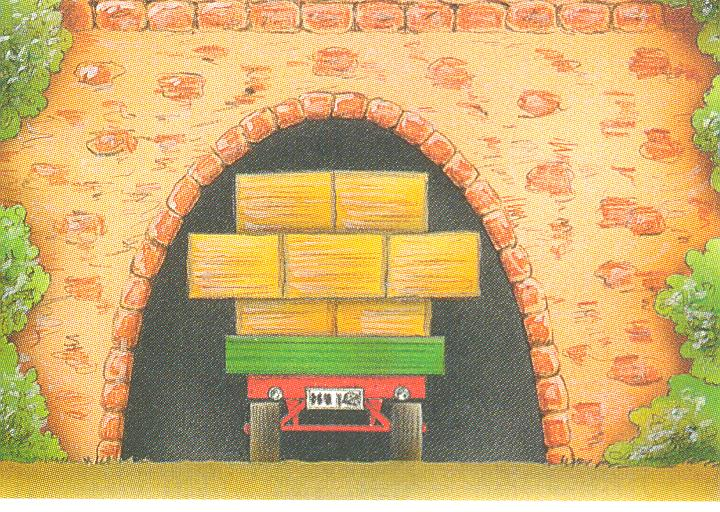
\includegraphics[scale=1]{tunnel.jpg}
\end{aufgabe}

\end{flushleft} 
\end{document}
